% Generated by pysimcount.pfchilds -- do not edit; regenerate instead.
% figure: main-total-all-formulas -- Every formula, X-Y-Z grouping, total gates vs n (cf. Childs et al. 2018 Fig. 3 right)
% source: ../np-main/aggregate.json + ../np-main-n9/seed{seed}, ../np-main-n11/seed{seed} (seeds [1, 2, 3, 4, 5, 6, 7, 8, 9, 10]); run commits: 01d3c275ceae2840002bd1aaea68f59b987c4975, e42ff29056ad9ea7fc7c9899fab334903e42e3e3
% metric=total kind=xyz merged (cz, simcount template)
% measured n: mean over seeds of the run's totals; bars min..max over seeds
% r from per-seed power-law fits (n = 5--11), mean count over seeds; r = ceil(a n^b); point=seed-mean; bars = min..max of per-seed fits
% per-step counts exactly affine in n (checked on n = [10, 20, 40], direct build at n = [100])
% shown: suzuki4, suzuki6, mo-q6, mo-q14, bm-q10, mo-o8-q21, morales-y8m10, morales-m8
% removed (see main-total-all-formulas-ranking.md): lie-trotter, suzuki2, suzuki8
% figure made at git_commit=e5d9ee696f892e28aced765585653760f8a427c4 git_dirty=False
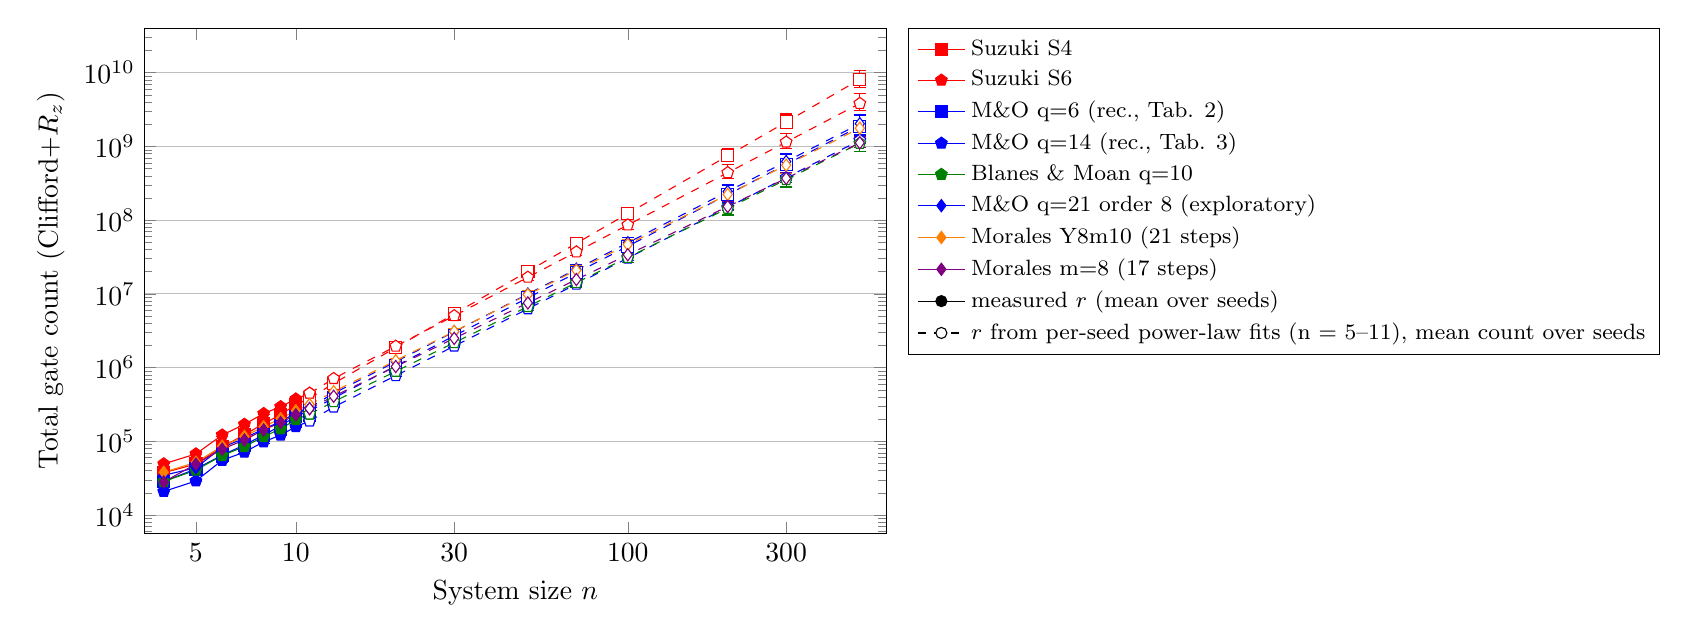
\begin{tikzpicture}
  \begin{loglogaxis}[
    width=11cm, height=8cm,
    xlabel={System size $n$},
    ylabel={Total gate count (Clifford+$R_z$)},
    xtick={5,10,30,100,300}, xticklabels={5,10,30,100,300},
    xmin=3.5, xmax=600,
    ymajorgrids=true,
    legend pos=outer north east,
    legend cell align=left,
    legend style={font=\footnotesize},
  ]
    % suzuki4: measured n, mean over seeds, bars min..max over seeds
    \addplot[red, solid, mark=square*, mark size=2.2pt, mark options={solid, fill=red}, error bars/.cd, y dir=both, y explicit, error bar style={solid}] coordinates {
      (4,37651.2) += (0,508.8) -= (0,339.2)
      (5,49184) += (0,1696) -= (0,1484)
      (6,84333.6) += (0,5978.4) -= (0,4197.6)
      (7,122578) += (0,9497.6) -= (0,8310.4)
      (8,174349) += (0,7123.2) -= (0,6444.8)
      (9,229914) += (0,10494) -= (0,12402)
      (10,315032) += (0,24168) -= (0,11872)
      (11,384780) += (0,16324) -= (0,9328)
    };
    \addlegendentry{Suzuki S4}
    % suzuki4: extrapolated, r = ceil(3.65267 n^1.59931), per step = 212 n + 0; bars min..max of per-seed fits
    \addplot[red, dashed, mark=square*, mark size=2.2pt, mark options={solid, fill=white}, forget plot, error bars/.cd, y dir=both, y explicit, error bar style={solid}] coordinates {
      (11,384780)
      (13,609903) += (0,26733.2) -= (0,20118.8)
      (20,1.86772e+06) += (0,137800) -= (0,103880)
      (30,5.3583e+06) += (0,550140) -= (0,410220)
      (50,2.02333e+07) += (0,2.86412e+06) -= (0,2.07548e+06)
      (70,4.85565e+07) += (0,8.13232e+06) -= (0,5.80244e+06)
      (100,1.22856e+08) += (0,2.39963e+07) -= (0,1.68773e+07)
      (200,7.46656e+08) += (0,1.8712e+08) -= (0,1.27955e+08)
      (300,2.14644e+09) += (0,6.08964e+08) -= (0,4.09718e+08)
      (500,8.12156e+09) += (0,2.64878e+09) -= (0,1.74725e+09)
    };
    % suzuki6: measured n, mean over seeds, bars min..max over seeds
    \addplot[red, solid, mark=pentagon*, mark size=2.2pt, mark options={solid, fill=red}, error bars/.cd, y dir=both, y explicit, error bar style={solid}] coordinates {
      (4,49536) += (0,0) -= (0,0)
      (5,67596) += (0,4644) -= (0,516)
      (6,121982) += (0,8049.6) -= (0,4334.4)
      (7,170486) += (0,10113.6) -= (0,11558.4)
      (8,238598) += (0,9081.6) -= (0,7430.4)
      (9,295358) += (0,11145.6) -= (0,16718.4)
      (10,375648) += (0,26832) -= (0,14448)
      (11,449539) += (0,15892.8) -= (0,6811.2)
    };
    \addlegendentry{Suzuki S6}
    % suzuki6: extrapolated, r = ceil(1.63295 n^1.35284), per step = 1032 n + 0; bars min..max of per-seed fits
    \addplot[red, dashed, mark=pentagon*, mark size=2.2pt, mark options={solid, fill=white}, forget plot, error bars/.cd, y dir=both, y explicit, error bar style={solid}] coordinates {
      (11,449539)
      (13,711048) += (0,40248) -= (0,13416)
      (20,1.95048e+06) += (0,154800) -= (0,72240)
      (30,5.05577e+06) += (0,578952) -= (0,287928)
      (50,1.68216e+07) += (0,2.6832e+06) -= (0,1.4448e+06)
      (70,3.71314e+07) += (0,7.00728e+06) -= (0,3.82872e+06)
      (100,8.60482e+07) += (0,1.89062e+07) -= (0,1.04026e+07)
      (200,4.40808e+08) += (0,1.24521e+08) -= (0,6.86693e+07)
      (300,1.14685e+09) += (0,3.66783e+08) -= (0,2.01642e+08)
      (500,3.82702e+09) += (0,1.40832e+09) -= (0,7.67653e+08)
    };
    % mo-q6: measured n, mean over seeds, bars min..max over seeds
    \addplot[blue, solid, mark=square*, mark size=2.2pt, mark options={solid, fill=blue}, error bars/.cd, y dir=both, y explicit, error bar style={solid}] coordinates {
      (4,28639.6) += (0,1720.4) -= (0,3339.6)
      (5,42251) += (0,2024) -= (0,4301)
      (6,65122.2) += (0,1669.8) -= (0,2884.2)
      (7,89435.5) += (0,4427.5) -= (0,6198.5)
      (8,122250) += (0,11334.4) -= (0,6881.6)
      (9,162350) += (0,8424.9) -= (0,12068.1)
      (10,219098) += (0,8602) -= (0,14168)
      (11,259376) += (0,27273.4) -= (0,22820.6)
    };
    \addlegendentry{M\&O q=6 (rec., Tab. 2)}
    % mo-q6: extrapolated, r = ceil(3.93927 n^1.32338), per step = 253 n + 0; bars min..max of per-seed fits
    \addplot[blue, dashed, mark=square*, mark size=2.2pt, mark options={solid, fill=white}, forget plot, error bars/.cd, y dir=both, y explicit, error bar style={solid}] coordinates {
      (11,259376)
      (13,387115) += (0,24009.7) -= (0,15458.3)
      (20,1.05197e+06) += (0,106766) -= (0,65274)
      (30,2.69749e+06) += (0,368874) -= (0,245916)
      (50,8.84108e+06) += (0,1.62046e+06) -= (0,1.08664e+06)
      (70,1.93375e+07) += (0,4.1282e+06) -= (0,2.76099e+06)
      (100,4.43307e+07) += (0,1.09498e+07) -= (0,7.29146e+06)
      (200,2.22463e+08) += (0,6.96509e+07) -= (0,4.57171e+07)
      (300,5.71785e+08) += (0,2.01864e+08) -= (0,1.30806e+08)
      (500,1.87899e+09) += (0,7.60176e+08) -= (0,4.83445e+08)
    };
    % mo-q14: measured n, mean over seeds, bars min..max over seeds
    \addplot[blue, solid, mark=pentagon*, mark size=2.2pt, mark options={solid, fill=blue}, error bars/.cd, y dir=both, y explicit, error bar style={solid}] coordinates {
      (4,20916) += (0,0) -= (0,0)
      (5,29050) += (0,0) -= (0,0)
      (6,55427.4) += (0,348.6) -= (0,3137.4)
      (7,71579.2) += (0,1626.8) -= (0,2440.2)
      (8,98537.6) += (0,3718.4) -= (0,5577.6)
      (9,121836) += (0,3660.3) -= (0,1568.7)
      (10,158032) += (0,4648) -= (0,1162)
      (11,189174) += (0,2556.4) -= (0,3834.6)
    };
    \addlegendentry{M\&O q=14 (rec., Tab. 3)}
    % mo-q14: extrapolated, r = ceil(1.412 n^1.28559), per step = 581 n + 0; bars min..max of per-seed fits
    \addplot[blue, dashed, mark=pentagon*, mark size=2.2pt, mark options={solid, fill=white}, forget plot, error bars/.cd, y dir=both, y explicit, error bar style={solid}] coordinates {
      (11,189174)
      (13,292301) += (0,2265.9) -= (0,5287.1)
      (20,778540) += (0,23240) -= (0,23240)
      (30,1.96088e+06) += (0,95865) -= (0,78435)
      (50,6.28642e+06) += (0,453180) -= (0,302120)
      (70,1.35553e+07) += (0,1.2079e+06) -= (0,744261)
      (100,3.06013e+07) += (0,3.27103e+06) -= (0,1.84177e+06)
      (200,1.49271e+08) += (0,2.08463e+07) -= (0,1.09925e+07)
      (300,3.77168e+08) += (0,6.03252e+07) -= (0,3.08337e+07)
      (500,1.21287e+09) += (0,2.24527e+08) -= (0,1.11e+08)
    };
    % bm-q10: measured n, mean over seeds, bars min..max over seeds
    \addplot[green!50!black, solid, mark=pentagon*, mark size=2.2pt, mark options={solid, fill=green!50!black}, error bars/.cd, y dir=both, y explicit, error bar style={solid}] coordinates {
      (4,28522.8) += (0,1501.2) -= (0,166.8)
      (5,40866) += (0,834) -= (0,1251)
      (6,64301.4) += (0,750.6) -= (0,1751.4)
      (7,84942.9) += (0,2627.1) -= (0,3210.9)
      (8,116093) += (0,7339.2) -= (0,6004.8)
      (9,148244) += (0,5629.5) -= (0,9382.5)
      (10,197658) += (0,2502) -= (0,5838)
      (11,234854) += (0,12843.6) -= (0,10091.4)
    };
    \addlegendentry{Blanes \& Moan q=10}
    % bm-q10: extrapolated, r = ceil(2.82314 n^1.2111), per step = 417 n + 0; bars min..max of per-seed fits
    \addplot[green!50!black, dashed, mark=pentagon*, mark size=2.2pt, mark options={solid, fill=white}, forget plot, error bars/.cd, y dir=both, y explicit, error bar style={solid}] coordinates {
      (11,234854)
      (13,345318) += (0,7047.3) -= (0,9215.7)
      (20,890712) += (0,35028) -= (0,48372)
      (30,2.17924e+06) += (0,135108) -= (0,177642)
      (50,6.7408e+06) += (0,619245) -= (0,736005)
      (70,1.41863e+07) += (0,1.54707e+06) -= (0,1.83897e+06)
      (100,3.12333e+07) += (0,4.0449e+06) -= (0,4.6704e+06)
      (200,1.44899e+08) += (0,2.45696e+07) -= (0,2.71384e+07)
      (300,3.55684e+08) += (0,6.85298e+07) -= (0,7.42093e+07)
      (500,1.10288e+09) += (0,2.45279e+08) -= (0,2.59291e+08)
    };
    % mo-o8-q21: measured n, mean over seeds, bars min..max over seeds
    \addplot[blue, solid, mark=diamond*, mark size=2.2pt, mark options={solid, fill=blue}, error bars/.cd, y dir=both, y explicit, error bar style={solid}] coordinates {
      (4,34720) += (0,0) -= (0,0)
      (5,43834) += (0,3906) -= (0,434)
      (6,83328) += (0,5208) -= (0,5208)
      (7,109976) += (0,5468.4) -= (0,6683.6)
      (8,147907) += (0,4860.8) -= (0,9027.2)
      (9,185144) += (0,2343.6) -= (0,5468.4)
      (10,243908) += (0,16492) -= (0,9548)
      (11,289304) += (0,6683.6) -= (0,2864.4)
    };
    \addlegendentry{M\&O q=21 order 8 (exploratory)}
    % mo-o8-q21: extrapolated, r = ceil(1.3736 n^1.30758), per step = 868 n + 0; bars min..max of per-seed fits
    \addplot[blue, dashed, mark=diamond*, mark size=2.2pt, mark options={solid, fill=white}, forget plot, error bars/.cd, y dir=both, y explicit, error bar style={solid}] coordinates {
      (11,289304)
      (13,447975) += (0,14669.2) -= (0,7898.8)
      (20,1.20652e+06) += (0,78120) -= (0,43400)
      (30,3.07012e+06) += (0,263004) -= (0,179676)
      (50,9.96898e+06) += (0,1.27162e+06) -= (0,898380)
      (70,2.16609e+07) += (0,3.37218e+06) -= (0,2.33926e+06)
      (100,4.93545e+07) += (0,9.14872e+06) -= (0,6.38848e+06)
      (200,2.44759e+08) += (0,5.93886e+07) -= (0,4.09522e+07)
      (300,6.24778e+08) += (0,1.73348e+08) -= (0,1.17779e+08)
      (500,2.03494e+09) += (0,6.56295e+08) -= (0,4.38253e+08)
    };
    % morales-y8m10: measured n, mean over seeds, bars min..max over seeds
    \addplot[orange, solid, mark=diamond*, mark size=2.2pt, mark options={solid, fill=orange}, error bars/.cd, y dir=both, y explicit, error bar style={solid}] coordinates {
      (4,38192) += (0,0) -= (0,0)
      (5,52080) += (0,0) -= (0,0)
      (6,85932) += (0,2604) -= (0,2604)
      (7,116659) += (0,4860.8) -= (0,1215.2)
      (8,158323) += (0,8332.8) -= (0,5555.2)
      (9,203893) += (0,7030.8) -= (0,8593.2)
      (10,260400) += (0,17360) -= (0,8680)
      (11,315084) += (0,9548) -= (0,9548)
    };
    \addlegendentry{Morales Y8m10 (21 steps)}
    % morales-y8m10: extrapolated, r = ceil(1.66328 n^1.25438), per step = 868 n + 0; bars min..max of per-seed fits
    \addplot[orange, dashed, mark=diamond*, mark size=2.2pt, mark options={solid, fill=white}, forget plot, error bars/.cd, y dir=both, y explicit, error bar style={solid}] coordinates {
      (11,315084)
      (13,472800) += (0,12412.4) -= (0,21439.6)
      (20,1.24645e+06) += (0,72912) -= (0,83328)
      (30,3.10136e+06) += (0,283836) -= (0,289044)
      (50,9.79104e+06) += (0,1.18916e+06) -= (0,1.24124e+06)
      (70,2.09257e+07) += (0,3.0137e+06) -= (0,3.0623e+06)
      (100,4.67678e+07) += (0,7.91616e+06) -= (0,7.88144e+06)
      (200,2.23423e+08) += (0,4.87816e+07) -= (0,4.65248e+07)
      (300,5.58089e+08) += (0,1.3796e+08) -= (0,1.2895e+08)
      (500,1.76907e+09) += (0,5.02485e+08) -= (0,4.58825e+08)
    };
    % morales-m8: measured n, mean over seeds, bars min..max over seeds
    \addplot[violet, solid, mark=diamond*, mark size=2.2pt, mark options={solid, fill=violet}, error bars/.cd, y dir=both, y explicit, error bar style={solid}] coordinates {
      (4,28160) += (0,0) -= (0,0)
      (5,49280) += (0,0) -= (0,0)
      (6,78566.4) += (0,1689.6) -= (0,2534.4)
      (7,104474) += (0,3942.4) -= (0,985.6)
      (8,143053) += (0,9011.2) -= (0,2252.8)
      (9,180576) += (0,3168) -= (0,3168)
      (10,229504) += (0,9856) -= (0,4224)
      (11,278010) += (0,8518.4) -= (0,6969.6)
    };
    \addlegendentry{Morales m=8 (17 steps)}
    % morales-m8: extrapolated, r = ceil(2.19247 n^1.17079), per step = 704 n + 0; bars min..max of per-seed fits
    \addplot[violet, dashed, mark=diamond*, mark size=2.2pt, mark options={solid, fill=white}, forget plot, error bars/.cd, y dir=both, y explicit, error bar style={solid}] coordinates {
      (11,278010)
      (13,409094) += (0,11897.6) -= (0,6406.4)
      (20,1.03629e+06) += (0,47872) -= (0,36608)
      (30,2.49427e+06) += (0,166848) -= (0,128832)
      (50,7.54688e+06) += (0,725120) -= (0,506880)
      (70,1.5671e+07) += (0,1.7248e+06) -= (0,1.18272e+06)
      (100,3.39891e+07) += (0,4.44928e+06) -= (0,3.01312e+06)
      (200,1.53176e+08) += (0,2.56397e+07) -= (0,1.68819e+07)
      (300,3.69558e+08) += (0,6.99494e+07) -= (0,4.53658e+07)
      (500,1.12147e+09) += (0,2.43936e+08) -= (0,1.55584e+08)
    };
    \addlegendimage{black, solid, mark=*, mark options={solid, fill=black}}
    \addlegendentry{measured $r$ (mean over seeds)}
    \addlegendimage{black, dashed, mark=*, mark options={solid, fill=white}}
    \addlegendentry{$r$ from per-seed power-law fits (n = 5--11), mean count over seeds}
  \end{loglogaxis}
\end{tikzpicture}
